\documentclass{article}
\usepackage{amsmath}
\usepackage{amsfonts}
\usepackage{cancel}
\usepackage{pgfplots}



\title{Differentiation in HKDSE}
\author{@borisonwong}
\date{March 15, 2022}
\begin{document}
\maketitle
\tableofcontents
\pagebreak
\section{Differentiation and Derivatives}
\subsection{Derivatives}
Derivative is a measure of rate of change
of a function. The derivative of a function
at certain point can be visualised as the
slope of tangent of the function at that
point.
\subsection{Differentiation}
The process of finding derivatives is
called differentiation, we can treat it
as an operation. To denote this operation,
we use the following symbols
\begin{equation*}
    \frac{df}{dx} =\frac{df( x)}{dx} =\frac{d}{dx} f( x) =f'( x) =f'
\end{equation*}
These are all symbols representing
differentiating the function
\textbf{$f(x)$ with respect to $x$}. Please take
note that we are finding how sensitive
does the function value $f(x)$ changes as
$x$ changes.


Sometimes, we may want to know the
derivative of a function at a \textbf{particular
point}, let's say $(x\index{0},f(x\index{0})$
we denote this particular derivative as
\begin{equation*}
    \frac{d}{dx}\Bigl|_{x=x_{0}} f( x) \ \text{or} \ f'(x_0)
\end{equation*}
But you should NEVER write in the
following form
\begin{gather*}
    \xcancel{\ \frac{d}{dx} f( x_{0})}\\
    \frac{d}{dx} f( x_{0}) \neq \frac{d}{dx}\Bigl|_{x=x_{0}} f( x)
\end{gather*}
This is because 
$\displaystyle\frac{d}{dx}f(x_0)$ is finding the
derivative of the function
$f(x_0)$ with respect to $x$.
For example, if $\displaystyle f(x)=x^2+x$, 
then $\displaystyle f(x_0)=x_0^2+x_0$, and in fact
$\displaystyle x_0^2+x_0$ is a constant function of $x$,
differentiating $\displaystyle x_0^2+x_0$ with respect
to $x$ is not difference to differentiating
a constant, which gives zero.

If we differentiate a function twice,
also called \textbf{second derivative}, 
we denote them as
\begin{equation*}
    \frac{d^{2} f}{dx^{2}} =\frac{d^{2} f( x)}{dx^{2}} =\frac{d^{2}}{dx^{2}} f( x) =f"( x) =f"
\end{equation*}
Similarly, NEVER write in the form
\begin{equation*}
    \xcancel{\frac{d}{dx}\frac{d}{dx} f(x)} \ \text{or} \ \xcancel{\left(\frac{d}{dx}\right)^{2} f(x)}
\end{equation*}
Similarly, the second derivative of a
function at a particular point
$x=x_0$ can be denoted by
\begin{equation*}
    \frac{d^{2}}{dx^{2}}\Bigl|_{x=0} f( x) \ \text{or} \ f"(x_0)
\end{equation*}
\subsection{First principle}
As mentioned in the chapter \textit{Limit and e},
we can use the concept of limit to find
the derivative of a function, this approach
is called the \textbf{First Principle}.
\begin{equation*}
\begin{aligned}
    \frac{d}{dx} f( x) & =\lim _{h\rightarrow 0}\frac{f( x+h) -f( x)}{h}
\end{aligned}
\end{equation*}
To find the derivative of a function at
a particular point $x=x_0$, we can use the form
\begin{equation*}
\begin{aligned}
    \frac{d}{dx}\Bigl|_{x=x_{0}} f( x) & =\lim _{h\rightarrow 0}\frac{f( x_{0} +h) -f( x_{0})}{h} & \text{(More common)}\\
     & =\lim _{x\rightarrow x_{0}}\frac{f( x) -f( x_{0})}{x-x_{0}} & 
\end{aligned}
\end{equation*}
In HKDSE, if you are told to perform
differentiation from first principles,
you have to use them, making use of other
differentiation rules will score you no
mark.
\clearpage
\pagebreak
\section{Differentiation rules}
\subsection{Differentiation of common functions}
\label{subsec:commonFunctions}
To start with, let's take a look at what
are the derivatives of some fundamental
functions in mathematics. In HKDSE,
most of the time, when the question
does not specify the use of first
principle, you only need to directly
apply differentiation rules to solve the
problem.
\subsubsection{Constant functions}
\begin{equation*}
    \frac{d}{dx} C=0
\end{equation*}
Here $C$ is a constant, which means it
does not vary as $x$ changes.\\
\textbf{Proof}
\begin{equation*}
    \begin{aligned}
    \frac{d}{dx} C & =\lim _{h\rightarrow 0}\frac{C-C}{h}\\
     & =\lim _{h\rightarrow 0} 0\\
     & =0
    \end{aligned}
\end{equation*}
\subsubsection{Power rule}
\begin{equation*}
    \begin{aligned}
    \frac{d}{dx} x^{n} & =nx^{n-1}
\end{aligned}
\end{equation*}
You can easily memorise the rule by
\textit{"bring down the power and subtract one
from power"}. Also, please note that $n$ is
a constant (does not vary with $x$)\\
\textbf{Proof (for $n\in\mathbb{Z}^{+}$)}
\begin{equation*}
\begin{aligned}
    \frac{d}{dx} x^{n} & =\lim _{h\rightarrow 0}\frac{( x+h)^{n} -x^{n}}{h} & \\
     & =\lim _{h\rightarrow 0}\frac{\left(\cancel{x^{n}} +C_{1}^{n} hx^{n-1} +C_{2}^{n} h^{2} x^{n-2} +\cdots +h^{n}\right)\cancel{-x^{n}}}{h} & \text{(Binomial Theorem)}\\
     & =\lim _{h\rightarrow 0}\frac{nhx^{n-1} +C_{2}^{n} h^{2} x^{n-2} +\cdots +h^{n}}{h} & \\
     & =\lim _{h\rightarrow 0} nx^{n-1} +C_{2}^{n} hx^{n-2} +\cdots +h^{n-1} & \\
     & =nx^{n-1} +0+0+\cdots +0 & \\
     & =nx^{n-1} & 
\end{aligned}
\end{equation*}
This rule is applicable to all
$n\in\mathbb{R}$, but the proof for
non-integral values of $n$ is not shown
here because it involves the use of
advanced techniques.
\subsubsection{Exponential functions}
\begin{equation*}
    \frac{d}{dx} e^{x} =e^{x}
\end{equation*}
\textbf{Proof}
\begin{equation*}
\begin{aligned}
    \frac{d}{dx} e^{x} & =\lim _{h\rightarrow 0}\frac{e^{x+h} -e^{x}}{h}\\
     & =e^{x}\lim _{h\rightarrow 0}\left(\frac{e^{h} -1}{h}\right)\\
     & =e^{x} \cdot 1\\
     & =e^{x}
\end{aligned}
\end{equation*}
\subsubsection{Logarithmic functions}
\begin{equation*}
    \frac{d}{dx}\ln x=\frac{1}{x}
\end{equation*}
\textbf{Proof}
\begin{equation*}
\begin{aligned}
    \frac{d}{dx}\ln x & =\lim _{h\rightarrow 0}\frac{\ln( x+h) -\ln x}{h}\\
     & =\lim _{h\rightarrow 0}\frac{\ln\left(\frac{x+h}{x}\right)}{h}\\
     & =\lim _{h\rightarrow 0}\ln\left[ 1+\left(\frac{1}{x}\right) h\right]^{\frac{1}{h}}\\
     & =\ln\left[\lim _{h\rightarrow 0}\left( 1+\left(\frac{1}{x}\right) h\right)^{\frac{1}{h}}\right]\\
     & =\ln\left[ e^{\frac{1}{x}}\right]\\
     & =\frac{1}{x}
\end{aligned}
\end{equation*}
\subsubsection{Trigonometric functions}
Sine function
\begin{equation*}
    \frac{d}{dx}\sin x=\cos x    
\end{equation*}
\textbf{Proof}
\begin{equation*}
\begin{aligned}
    \frac{d}{dx}\sin x & =\lim _{h\rightarrow 0}\frac{\sin( x+h) -\sin x}{h} & \\
     & =\lim _{h\rightarrow 0}\frac{2\cos\frac{2x+h}{2}\sin\frac{h}{2}}{h} & \text{(Sum to product)}\\
     & =\left[\lim _{h\rightarrow 0}\cos\left( x+\frac{h}{2}\right)\right]\left[\lim _{\frac{h}{2}\rightarrow 0}\frac{\sin\frac{h}{2}}{\frac{h}{2}}\right] & \\
     & =\cos( x+0) \cdot 1 & \\
     & =\cos x & 
\end{aligned}
\end{equation*}
Cosine function
\begin{equation*}
    \frac{d}{dx}\cos x=\sin x    
\end{equation*}
\textbf{Proof}
\begin{equation*}
\begin{aligned}
    \frac{d}{dx}\cos x & =\lim _{h\rightarrow 0}\frac{\cos( x+h) -\cos x}{h} & \\
     & =\lim _{h\rightarrow 0}\frac{-2\sin\frac{2x+h}{2}\sin\frac{h}{2}}{h} & \text{(Sum to product)}\\
     & =-\left[\lim _{h\rightarrow 0}\sin\left( x+\frac{h}{2}\right)\right]\left[\lim _{\frac{h}{2}\rightarrow 0}\frac{\sin\frac{h}{2}}{\frac{h}{2}}\right] & \\
     & =-\sin( x+0) \cdot 1 & \\
     & =-\sin x & 
\end{aligned}
\end{equation*}
Tangent function
\begin{equation*}
    \frac{d}{dx}\tan x=\sec^{2} x
\end{equation*}
\textbf{Proof}
\begin{equation*}
\begin{aligned}
    \frac{d}{dx}\tan x & =\lim _{h\rightarrow 0}\frac{\tan( x+h) -\tan x}{h} & \\
    & =\lim _{h\rightarrow 0}\frac{1}{h}\left[\frac{\sin( x+h)}{\cos( x+h)} -\frac{\sin x}{\cos x}\right] & \\
    & =\lim _{h\rightarrow 0}\frac{1}{h}\left[\frac{\sin( x+h)\cos x-\cos( x+h)\sin x}{\cos( x+h)\cos x}\right] & \\
    & =\lim _{h\rightarrow 0}\frac{1}{h}\left[\frac{\sin( x+h-x)}{\cos( x+h)\cos x}\right] & \text{(Double angle formula)}\\
    & =\left[\lim _{h\rightarrow 0}\frac{\sin h}{h}\right]\left[\lim _{h\rightarrow 0}\frac{1}{\cos( x+h)\cos x}\right] & \\
    & =1\cdot \frac{1}{\cos( x+0)\cos x} & \\
    & =\sec^{2} x & 
\end{aligned}
\end{equation*}
\subsubsection{Summary}
\begin{equation*}
\begin{aligned}
    &\frac{d}{dx} C =0 &   &\frac{d}{dx} x^{n} =nx^{n-1}\\
    &\frac{d}{dx} e^{x} =e^{x} &  &\frac{d}{dx}\ln x =\frac{1}{x}\\
    &\frac{d}{dx}\sin x =\cos x &  &\frac{d}{dx}\cos x =-\sin x\\
    &\frac{d}{dx}\tan x =\sec^{2} x
\end{aligned}
\end{equation*}
\subsection{Differentiating the sum, product and quotient of functions}
In this part, we will look at functions that are constructed from the fundamental functions in \ref{subsec:commonFunctions}
\subsubsection{Addition/subtraction rule}
\begin{gather*}
    \frac{d}{dx}[ f( x) \pm g( x) =\frac{d}{dx} f( x) \pm \frac{d}{dx} g( x)\\
    \frac{d}{dx} kf( x) =k\frac{d}{dx} f( x)
\end{gather*}
\textbf{Proof}
\begin{equation*}
\begin{aligned}
    \frac{d}{dx}[ f( x) \pm g( x)] & =\lim _{h\rightarrow 0}\frac{[ f( x+h) \pm g( x+h)] -[ f( x) \pm g( x)]}{h}\\
        & =\lim _{h\rightarrow 0}\frac{f( x+h) -f( x)}{h} \pm \lim _{h\rightarrow 0}\frac{g( x+h) -g( x)}{h}\\
        & =\frac{d}{dx} f( x) \pm \frac{d}{dx} g( x)\\
    \frac{d}{dx} kf( x) & =\lim _{h\rightarrow 0}\frac{kf( x+h) -kf( x)}{h}\\
        & =k\lim _{h\rightarrow 0}\frac{f( x+h) -f( x)}{h}\\
        & =k\frac{d}{dx} f( x)
\end{aligned}
\end{equation*}
\textbf{Example}
\begin{equation*}
\begin{aligned}
    \frac{d}{dx}\left(\sin x+x^{2} +\ln x+e^{x}\right) & =\frac{d}{dx}\sin x+\frac{d}{dx} x^{2} +\frac{d}{dx}\ln x+\frac{d}{dx} e^{x}\\
    & =\cos x+2x+\frac{1}{x} +e^{x}
\end{aligned}
\end{equation*}
Note: When you have more experiences
in differentiation, you will be able to
directly compute the derivative.
\subsubsection{Product rule}
\begin{equation*}
    \frac{d}{dx} f( x) g( x) =f( x)\frac{d}{dx} g( x) +g( x)\frac{d}{dx} f( x)
\end{equation*}
\textbf{Proof}
\begin{equation*}
\begin{aligned}
\frac{d}{dx} f( x) g( x) & =\lim _{h\rightarrow 0}\frac{f( x+h) g( x+h) -f( x) g( x)}{h}\\
 & = \lim_{h\rightarrow 0}\frac{f(x+h)g(x+h)+f(x+h)g(x)-f(x+h)g(x)-f(x)f(x)}{h}\\
 & =\lim _{h\rightarrow 0}\frac{f( x+h)[ g( x+h) -g( x)] +g( x)[ f( x+h) -f( x)]}{h}\\
 & =\left[\lim _{h\rightarrow 0} f( x+h)\right]\left[\lim _{h\rightarrow 0}\frac{g( x+h) -g( x)}{h}\right] +\left[\lim _{h\rightarrow 0} g( x)\right]\left[\lim _{h\rightarrow 0}\frac{f( x+h) -f( x)}{h}\right]\\
 & =f( x+0)\frac{d}{dx} g( x) +g( x)\frac{d}{dx} f( x)\\
 & =f( x)\frac{d}{dx} g( x) +g( x)\frac{d}{dx} f( x)
\end{aligned}
\end{equation*}
\textbf{Example}
\begin{equation*}
\begin{aligned}
    \frac{d}{dx}\sin x\ln x & =\sin x\frac{d}{dx}\ln x+\ln x\frac{d}{dx}\sin x\\
     & =\frac{\sin x}{x} +\cos x\ln x
\end{aligned}
\end{equation*}
\subsubsection{Quotient rule}
\begin{equation*}
    \frac{d}{dx}\left[\frac{f( x)}{g( x)}\right] =\frac{g( x)\frac{d}{dx} f( x) -f( x)\frac{d}{dx} g( x)}{[ g( x)]^{2}}
\end{equation*}
Note: This rule is very messy, I seldom
use it when performing differentiation.
You are advised to use the product rule
in conjunction with negative powers to
handle it.\\
\textbf{Proof}
\begin{equation*}
\begin{aligned}
    \frac{d}{dx}\left[\frac{f( x)}{g( x)}\right] & =\lim _{h\rightarrow 0}\frac{\frac{f( x+h)}{g( x+h)} -\frac{f( x)}{g( x)}}{h}\\
    & =\lim _{h\rightarrow 0}\frac{1}{h}\left[\frac{f( x+h) g( x) -f( x) g( x+h)}{g( x+h) g( x)}\right]\\
    & =\lim _{h\rightarrow 0}\frac{1}{h}\left[\frac{f( x+h) g( x) +f( x) g( x) -f( x) g( x) -f( x) g( x+h)}{g( x+h) g( x)}\right]\\
    & =\lim _{h\rightarrow 0}\frac{1}{h}\left[\frac{g( x)[ f( x+h) -f( x)] -f( x)[ g( x+h) -g( x)]}{g( x+h) g( x)}\right]\\
    & =\left[\lim _{h\rightarrow 0}\frac{1}{g( x+h) g( x)}\right]\left[ g( x)\lim _{h\rightarrow 0}\frac{f( x+h) -f( x)}{h} -f( x)\lim _{h\rightarrow 0}\frac{g( x+h) -g( x)}{h}\right]\\
    & =\frac{1}{g( x+0) g( x)}\left[ g( x)\frac{d}{dx} f( x) -f( x)\frac{d}{dx} g( x)\right]\\
    & =\frac{g( x)\frac{d}{dx} f( x) -f( x)\frac{d}{dx} g( x)}{[ g( x)]^{2}}
\end{aligned}
\end{equation*}
\textbf{Example}
\begin{equation*}
\begin{aligned}
    \frac{d}{dx}\left[\frac{\sin x}{\sqrt{x}}\right] & =\frac{\sqrt{x}\frac{d}{dx}\sin x-\sin x\frac{d}{dx} x^{\frac{1}{2}}}{\left(\sqrt{x}\right)^{2}}\\
    & =\frac{\sqrt{x}\cos x-(\sin x)\left(\frac{1}{2\sqrt{x}}\right)}{x}\\
    & =\frac{\cos x}{\sqrt{x}} -\frac{\sin x}{2x\sqrt{x}}
\end{aligned}
\end{equation*}
Alternative method:
\begin{equation*}
\begin{aligned}
    \frac{d}{dx}\left[\frac{\sin x}{\sqrt{x}}\right] & =\frac{d}{dx}(\sin x) x^{-\frac{1}{2}}\\
    & =\sin x\frac{d}{dx} x^{-\frac{1}{2}} +x^{-\frac{1}{2}}\frac{d}{dx}\sin x\\
    & =(\sin x)\left(\frac{-1}{2} x^{-\frac{3}{2}}\right) +x^{-\frac{1}{2}}\cos x\\
    & =\frac{\cos x}{\sqrt{x}} -\frac{\sin x}{2x\sqrt{x}}
\end{aligned}
\end{equation*}
The alternative method seems more indirect,
 but it is helpful when dealing with more
 complex functions. The chances of
 confusing with $+$ or $–$ sign in quotient rule
 is reduced.
\subsection{Chain rule and composite functions}
\begin{equation*}
    \frac{dy}{dx} =\left(\frac{dy}{du}\right)\left(\frac{du}{dx}\right)
\end{equation*}
This representation may seem abstract to
you, recall what we have discussed before,
the notation $\displaystyle  \frac{dy}{dx}$ means
differentiating function $y$ with respect to $x$.
Similarly, $\displaystyle  \frac{dy}{du}$ means
differentiating function $y$ with respect
to $u$. And $\displaystyle  \frac{du}{dx}$ means
differentiating $u$ with respect to $x$.\\
\textbf{Worked Example 1}\\
Let $\displaystyle  y=\sin{2x}$, find $\displaystyle  \frac{dy}{dx}$\\
\textbf{Solution}\\
We may set $u=2x$ and see what happens
\begin{equation*}
\begin{aligned}
    \frac{dy}{dx} & =\frac{d(\sin 2x)}{dx}\\
    & =\frac{d(\sin u)}{dx}
\end{aligned}
\end{equation*}
Remember, we cannot apply the rule
$\displaystyle \frac{d}{dx}\sin{x}=\cos{x}$
directly, this is because we the variable
in the function is $u$ but we are
differentiating with respect to $x$,
therefore, we can apply the chain rule.
\begin{equation*}
\begin{aligned}
    \frac{d(\sin u)}{dx} & =\frac{d(\sin u)}{du} \cdot \frac{du}{dx}
\end{aligned}
\end{equation*}
Now, we can apply the rule $\frac{d}{du}\sin{u}=\cos{u}$
\begin{equation*}
\begin{aligned}
    \frac{d(\sin u)}{dx} & =\cos u\cdot \frac{du}{dx}
\end{aligned}
\end{equation*}
So what is $\displaystyle \frac{du}{dx}$? Recall
$u=2x$, so $\displaystyle \frac{du}{dx}=\frac{d(2x)}{dx}$.
\begin{equation*}
\begin{aligned}
    \frac{d}{dx}\sin 2x & =\cos 2x\cdot 2\\
    & =2\cos 2x
\end{aligned}
\end{equation*}
In practice, the chain can be quite long,
and in fact you can make it as long as
you like. The essence of chain rule is
it helps you differentiate the right
function with respect to the right
variable.
\begin{equation*}
    \frac{dy}{dx} =\frac{dy}{du} \cdot \frac{du}{dh} \cdot \frac{dh}{dk} \cdots \frac{dn}{dx}
\end{equation*}
From time to time, you may find the use
of substitution annoying and time
consuming, you may want to adopt a
more straight forward approach.
\begin{equation*}
    \frac{d}{dx} f[ g( x)] =f'[ g( x)]\frac{d}{dx} g( x)
\end{equation*}
What we are doing here is first find
out the derivative of
$f(x)$, which is $f'(x)$ then put
$x=g(x)$ to $f'(x)$, that gives
$f'[g(x)]$. Then differentiate
$g(x)$ with respect to $x$.\\
\textbf{Worked Example 2}\\
Find $\displaystyle \frac{d}{dx}\sin{2x}$\\
\textbf{Solution}\\
First, we identify $g(x)=2x$,
$f(x)=\sin{x}$, therefore
$f[g(x)]=\sin{2x}$.\\
Then, we ask ourselves what is
$f'(x)$, obviously, $\displaystyle f'(x)=\frac{d}{dx}\sin{x}=\cos{x}$.\\
We then know $f'[g(x)]=\cos{2x}$\\
Lastly, we want to know what is
$\displaystyle \frac{d}{dx}g(x)$, obviously,
$\displaystyle \frac{d}{dx}2x=2$\\
Assemble what we have, we see
\begin{equation*}
\begin{aligned}
    \frac{d}{dx}\sin 2x & =\cos 2x\cdot 2\\
    & =2\cos 2x
\end{aligned}
\end{equation*}
\textbf{Worked Example 3}
Many candidates are confused with what to
differentiate first and the relationship
among functions. I will suggest them to
spend some time to dissect what composes
the given function. For example,
consider
\begin{equation*}
\begin{aligned}
    y & =\sqrt{1+\sin\left( x^{2} +x+1\right)}
\end{aligned}
\end{equation*}
First of all, we see the innermost function is
\begin{equation*}
    x^{2} +x+1
\end{equation*}
Then we put it into a sine function and add it by 1
\begin{equation*}
    1+\sin\left( x^{2} +x+1\right)
\end{equation*}
Finally we take square root of it
\begin{equation*}
    \sqrt{1+\sin\left( x^{2} +x+1\right)}
\end{equation*}
So if we count from the outermost function,
the order is $\displaystyle \sqrt{}\rightarrow 1+\sin\rightarrow x^{2} +x+1$\\
Therefore, when performing chain rule,
the order of differentiation is $\displaystyle \sqrt{}\rightarrow 1+\sin\rightarrow x^{2} +x+1$.
\begin{equation*}
\begin{aligned}
    \frac{d}{dx}\sqrt{1+\sin\left( x^{2} +x+1\right)} & =\underbrace{\frac{1}{2\sqrt{1+\sin\left( x^{2} +x+1\right)}}}_{\text{differentiating} \ \sqrt{}} \cdot \underbrace{\cos\left( x^{2} +x+1\right)}_{\text{differentiating} \ 1+\sin} \cdot \underbrace{( 2x+1)}_{\text{differentiating} \ x^{2} +x+1}\\
    & =\frac{( 2x+1)\cos\left( x^{2} +x+1\right)}{2\sqrt{1+\sin\left( x^{2} +x+1\right)}}
\end{aligned}
\end{equation*}
\clearpage
\pagebreak
\noindent\textbf{Concept check (This type of question never appeared in HKCEE / HKALE / HKDSE)}\\
The following table gives some information about $f(x)$ and $g(x)$.
\begin{table}[!h]
    \centering
\begin{tabular}{|p{0.20\textwidth}|p{0.20\textwidth}|p{0.20\textwidth}|p{0.20\textwidth}|p{0.20\textwidth}|}
\hline 
\begin{center}
\end{center}
& \begin{center}
$\displaystyle f( x)$
\end{center}
& \begin{center}
$\displaystyle f'( x)$
\end{center}
& \begin{center}
$\displaystyle g( x)$
\end{center}
& \begin{center}
$\displaystyle g'( x)$
\end{center}
\\
\hline 
\begin{center}
$\displaystyle x=0$
\end{center}
& \begin{center}
1
\end{center}
& \begin{center}
2
\end{center}
& \begin{center}
1
\end{center}
& \begin{center}
1
\end{center}
\\
\hline 
\begin{center}
$\displaystyle x=1$
\end{center}
& \begin{center}
2
\end{center}
& \begin{center}
3
\end{center}
& \begin{center}
0
\end{center}
& \begin{center}
2
\end{center}
\\
\hline 
\begin{center}
$\displaystyle x=2$
\end{center}
& \begin{center}
3
\end{center}
& \begin{center}
4
\end{center}
& \begin{center}
1
\end{center}
& \begin{center}
3
\end{center}
\\
\hline
\end{tabular}
    
\end{table}\\
Find $\displaystyle \frac{d}{dx}\Bigl|_{x=1} f[ g( x)]$\\
\textbf{Solution}\\
By chain rule, we see
\begin{equation*}
\begin{aligned}
    \frac{d}{dx} f[ g( x)] & =f'[ g( x)] g'( x)\\
    \frac{d}{dx}\Bigl|_{x=1} f[ g( x)] & =f'[ g( 1)] g'( 1)\\
    & =f'( 0) \cdot 2\\
    & =2\cdot 2=4
\end{aligned}
\end{equation*}
\pagebreak
\section{Advanced Differentiation Techniques}
\subsection{Implicit differentiation}
Previously, we often see equations in the
form $y=f(x)$, $y$ can be
expressed in terms of $x$ easily. However,
some relationships between $x$ and $y$ can
hardly (or impossible) to be represented
in this way, for example
\begin{equation*}
    e^{xy} +\sin y=1
\end{equation*}
Therefore, we apply the concept of chain
rule to find the derivatives of the
function. It may seem abstract to you,
let us start with some examples.\\
\textbf{Example 1}\\
Find $\displaystyle \frac{dy}{dx}$ if
$\displaystyle x^{2} +y^{2} =25$\\
 (Obviously it is the equation of circle which origin lies at (0,0) with radius 5)
 Hence, find $\displaystyle \frac{dy}{dx}\Bigl|_{x=3,y=4}$\\
\begin{center}
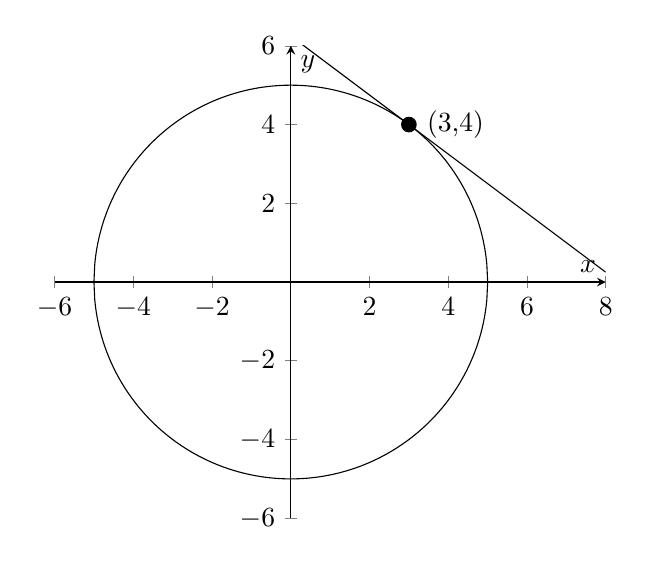
\begin{tikzpicture}
\begin{axis}[
    axis lines = center,
    xlabel = \(x\),
    ylabel = {\(y\)},
    xmax = 8, ymax = 6,
    xmin = -6, ymin = -6,
    x= 0.5 cm, y = 0.5 cm
]
%Below the red parabola is defined
\addplot [
    domain=-5:5, 
    samples=500
]{sqrt(25-x^2)};
\addplot [
    domain=-5:5, 
    samples=500
]{-sqrt(25-x^2)};
\addplot[
    domain=-5:8,
    samples = 100
]{(-3/4)*(x-3)+4};
\node[label={0:{(3,4)}},circle,fill,inner sep=2pt] at (axis cs:3,4) {};
\end{axis}
\end{tikzpicture}
\end{center}
\textbf{Solution}\\
\begin{equation*}
\begin{aligned}
    x^{2} +y^{2} & =25 & \\
    \frac{d}{dx}\left( x^{2} +y^{2}\right) & =\frac{d}{dx} 25 & \text{(differentiating both sides w.r.t.} \ x\text{)}\\
    2x+2y\left(\frac{dy}{dx}\right) & =0 & \text{(apply chain rule)}\\
    \frac{dy}{dx} & =-\frac{x}{y} & 
\end{aligned}
\end{equation*}
Hence, we see $\displaystyle \frac{dy}{dx}\Bigl|_{x=3,y=4} =-\frac{3}{4}$\\
\clearpage
\pagebreak
\noindent\textbf{Example 2}
Find $\displaystyle\frac{dy}{dx}$ if $e^{xy}+\sin{y}=1$.\\
\textbf{Solution}\\
\begin{equation*}
\begin{aligned}
    e^{xy} +\sin y & =1\\
    e^{xy}\left( x\frac{dy}{dx} +y\right) +\cos y\left(\frac{dy}{dx}\right) & =0\\
    xe^{xy}\left(\frac{dy}{dx}\right) +ye^{xy} +\cos y\left(\frac{dy}{dx}\right) & =0\\
    \left( xe^{xy} +\cos y\right)\frac{dy}{dx} & =-ye^{xy}\\
    \frac{dy}{dx} & =-\frac{ye^{xy}}{xe^{xy} +\cos y}
\end{aligned}
\end{equation*}
\subsection{Differentiation of inverse functions}
Inverse functions (denoted as $\displaystyle f^{-1}( x)$
for $f(x)$ means we can find back what value of $x$ gives
a particular function value $f(x)$. i.e.
if $f(a)=b,f^{-1}(b)=a$. Or we can refer to a common example
\begin{equation*}
\begin{aligned}
    \sin\left(\frac{\pi }{6}\right) & =\frac{1}{2}\\
    \sin^{-1}\left(\frac{1}{2}\right) & =\frac{\pi }{6}
\end{aligned}
\end{equation*}
Note: Of course $\displaystyle \sin^{-1}\left(\frac{1}{2}\right) =\frac{\pi }{6} ,\frac{5\pi }{6} \cdots $
But in this context we consider $\displaystyle x=\sin^{-1} y$
for $\displaystyle x\in \left[ -\frac{\pi }{2} ,\frac{\pi }{2}\right]$
only. The reason behind this assumption is
not emphasised here. I just want to give
you some fundamental concepts about
inverse functions.
Back to the topic, how we can differentiate
inverse functions like $\displaystyle y=\sin^{-1} x$
with respect to $x$?\\
\textbf{Example 1}
\begin{equation*}
\begin{aligned}
    y & =\sin^{-1} x & \\
    \sin y & =x & ( 1)\\
    \cos y\left(\frac{dy}{dx}\right) & =1 & \text{(differentiating both sides w.r.t.} \ x\text{)}\\
    \frac{dy}{dx} & =\frac{1}{\cos y} & \\
    \frac{dy}{dx} & =\frac{1}{\sqrt{1-\sin^{2} y}} & \text{(Remember} \ \sin^{2} y+\cos^{2} y=1\text{)}\\
    \frac{d}{dx}\sin^{-1} x & =\frac{1}{\sqrt{1-x^{2}}} & \text{(Using} \ ( 1) \ \text{)}
\end{aligned}
\end{equation*}
\clearpage
\pagebreak
\subsection{Logarithmic differentiation}
Some functions are hard to be differentiated
(especially those involving non-constant
powers and multiplication of lengthy
functions). For these cases, we may
first take natural logarithm to both
sides, then differentiate both sides.\\
\textbf{Example 1}
\begin{equation*}
\begin{aligned}
    y & =\left( x^{2} +x+1\right)^{x} & \\
    \ln y & =\ln\left( x^{2} +x+1\right)^{x} & \\
    \ln y & =x\ln\left( x^{2} +x+1\right) & \text{(remember} \ \ln a^{b} =b\ln a\text{)}\\
    \frac{1}{y}\left(\frac{dy}{dx}\right) & =\frac{d}{dx} x\ln\left( x^{2} +x+1\right) & \text{(differentiating both sides w.r.t.} \ x\text{)}\\
    \frac{1}{y}\left(\frac{dy}{dx}\right) & =x\left(\frac{2x+1}{x^{2} +x+1}\right) +\ln\left( x^{2} +x+1\right) & \\
    \frac{dy}{dx} & =y\left[ x\left(\frac{2x+1}{x^{2} +x+1}\right) +\ln\left( x^{2} +x+1\right)\right] & \\
    & =\left( x^{2} +x+1\right)^{x}\left[\frac{x( 2x+1)}{x^{2} +x+1} +\ln\left( x^{2} +x+1\right)\right] & 
\end{aligned}
\end{equation*}
\textbf{Example 2}
\begin{equation*}
\begin{aligned}
    y & =\frac{( x+1)\left( x^{2} +1\right)^{2}}{x-1}
\end{aligned}
\end{equation*}
In fact, we can use product rules and
quotient rules to differentiate the
function, but it takes plenty of time.
Logarithmic differentiation provides
an alternative to us.
\begin{equation*}
\begin{aligned}
    y & =\frac{( x+1)\left( x^{2} +1\right)^{2}}{x-1}\\
    \ln y & =\ln( x+1) +2\ln\left( x^{2} +1\right) -\ln( x-1)\\
    \frac{1}{y}\left(\frac{dy}{dx}\right) & =\frac{1}{x+1} +\frac{2( 2x)}{x^{2} +1} -\frac{1}{x-1}\\
    \frac{dy}{dx} & =\frac{( x+1)\left( x^{2} +1\right)^{2}}{x-1}\left[\frac{1}{x+1} +\frac{4x}{x^{2} +1} -\frac{1}{x-1}\right]
\end{aligned}
\end{equation*}
But remember this method does not provide
a simplified form of the answer,
further manipulation is required.
However, if the question only asks
$\displaystyle \frac{dy}{dx}\Bigl|_{x=0}$
, we can directly substitute$x=0$ to the result.
\begin{equation*}
\begin{aligned}
    \frac{dy}{dx}\Bigl|_{x=0} & =\frac{( 0+1)\left( 0^{2} +1\right)^{2}}{0-1}\left[\frac{1}{0+1} +\frac{4( 0)}{0^{2} +1} -\frac{1}{0-1}\right]\\
    & =-1( 1+1)\\
    & =-2
\end{aligned}
\end{equation*}
\subsection{Differentiation by calculator}
If you have not owned fx–3650P II / fx–3650P calculators, purchase one.\\
The aforementioned calculators allow us
to check the derivative of a function at
a certain point. The button can be found
at the RHS of "Prog". To call the function,
press \textbf{SHIFT} then $\int$ \textbf{dx}.\\
You should see \textbf{d/dX (}, The syntax of the operator is
\textbf{d/dX(function,value)}.\\
For example, to calculate
\begin{equation*}
    \frac{d}{dx}\Bigl|_{x=0}\frac{( x+1)\left( x^{2} +1\right)^{2}}{x-1}
\end{equation*}
The output is –2, which means $\displaystyle \frac{d}{dx}\Bigl|_{x=0}\frac{( x+1)\left( x^{2} +1\right)^{2}}{x-1} =-2$
\end{document}
